\documentclass[a4paper,11pt]{article}
\usepackage[utf8]{inputenc}
\usepackage[OT1]{fontenc}
\usepackage[english]{babel}
\usepackage[margin=1.2in]{geometry}
\usepackage{graphicx}
\usepackage{amsmath}
\usepackage{cite}
\usepackage[perpage,symbol]{footmisc}
\usepackage[hang,small]{caption}
\usepackage{parskip}
\usepackage{array}
\usepackage{pstricks}
\usepackage{pslatex}

%\usepackage{fancyvrb}

\author{Simon Mitternacht} 
\date{\today} 
\title{Sasalib: an open source C library for solvent accessible surface
  calculations}

\begin{document}
\maketitle
\hrule\vspace{0.5cm}
\noindent
The program/library Sasalib, including this manual, is licensed under
GPLv3, and can be downloaded from github at: 
\begin{center}
\texttt{https://github.com/mittinatten/sasalib/}
\end{center}
NB: This document is a draft slowly approaching completeness.
\vspace{0.5cm}
\hrule
\section{Introduction}
The Solvent Accessible Surface Area (SASA) of a molecule gives a
measure of the surface of the molecule in contact with solvent. This
area can for example quantify how folded the conformation of a
macromolecule is, and can also be used to compare the exposed
hydrophobic surfaces of different conformations or different
molecules. To define the SASA, $A$, of a given molecule, let a
spherical probe roll over the surface of the molecule, including
internal cavities. $A$ is then the surface drawn by the center of the
probe.~\cite{LnR} The probe represents a solvent molecule
(i.e.\ water). Cavities smaller than the solvent molecule do not
contribute to $A$.

Calculating Solvent Accessible Surface Areas (SASA) is a
run-of-the-mill calculation in protein structure studies. To the
author's knowledge there are no fully open source standalone programs
for doing this. Neither are there any libraries designed to be easily
integrated in other programs. The present library is an attempt to
resolve both these issues, and is released under the GNU General
Public License 3\footnote{See
  \texttt{http://www.gnu.org/licenses/gpl.html}}.

Sasalib is a both a standalone command line program and a C library
for protein SASA calculations. The library provides a simple interface
that takes PDB-files as input. It has default parameters to allow
straightforward calculations, but also allows the user to change most
parameters of the calculation. In addition, the user can treat the
calculation as a purely mathematical operation on a set of spheres, by
providing arbitrary coordinates and radii. Both Lee \& Richards'
\cite{LnR} and Shrake \& Rupley's \cite{SnR} algorithms are
available. They will be referred to as L\&R and S\&R throughout this
document. Future versions of the library might include other
algorithms as well.

In constructing the library three possible use cases were considered. 
\begin{enumerate}
\item The user has a PDB-file and wishes to calculate the total SASA of
  the structure, or the SASA for certain groups or types of atoms.
\item The user has a set of cartesian atom coordinates and radii for
  these atoms, and wants to calculate the total SASA for this object.
\item The user is simulating different conformations of a molecule and
  wants to measure the SASA at certain intervals during the simulation.
\end{enumerate}
For case 1 both the command-line interface (CLI) and the application
programming interface (API) can be used. Using the API gives more
flexibility in interpreting and analyzing the results. The other 2
cases can only be handled through the API. Both the API and the CLI
allow the user to set parameters for the calculation. 

A lot of the internals of the library are involved with classification
and categorization of atoms, which is necessary for assigning radii
and to present SASA values integrated over different atom types, amino
acid types, etc. If the user wants Sasalib to classify atoms and
assign radii, data must be provided in the PDB-format. Users can also
provide their own radii and coordinates, and get the SASA for each
individual atom.

This document is organized as follows. Section \ref{sec:howto_short}
gives a brief introduction to the library, presenting the command line
interface and a short sample program that gives a general idea of how
to use the library. The introduction is intended to cover most casual
users' needs. Section \ref{sec:alg} describes the algorithms and
compares their performance in terms of computational cost and
precision. In section \ref{sec:imp} the implementations are
described. Finally, section \ref{sec:using} gives a detailed
description of the API.

\section{Getting started}\label{sec:howto_short}

The source files \texttt{calc\_sasa.c} and \texttt{example.c} contain
a complete command-line interface and a minimal program to illustrate
how to use the library interface, respectively. 

\subsection{Installation} \label{sec:installing}

The repository can be cloned from github, either by using git directly
with the command
\begin{verbatim}
    $ git clone https://github.com/mittinatten/sasalib.git
\end{verbatim}
or by downloading the zipped archive from
\begin{verbatim}
    https://github.com/mittinatten/sasalib/archive/master.zip
\end{verbatim}
Sasalib itself only depends on regular C and GNU libraries, and should
therefore be straightforward to compile and install. Installation is
done by the regular sequence \verb|./configure|, \verb|make| and
\verb|make install|. Several versions of the GNU C Compiler and
Clang/LLVM have been tested successfully on both Linux and Mac OS X
platforms. The test-suite depends on the Check unit testing
framework\footnote{\texttt{http://check.sourceforge.net/}}.

\subsection{Command-line interface}

Compilation creates the binary \verb|calc_sasa| from
\verb|main.c|, which can be used to calculate the SASA of a
PDB-file. The simplest program call, with default parameters would be
\begin{verbatim}
    $ ./calc_sasa PDB-file
\end{verbatim}
Or, from STDIN:
\begin{verbatim} 
    $ ./calc_sasa < PDB-file    
\end{verbatim}
STDIN is only read if no file is specified.  By default the Shrake \&
Rupley algorithm is used, with 100 test points. 

\subsubsection{Options}
The following options are available
\begin{itemize}
  \item[-h] Prints help message.
  \item[-p] Probe radius. Default is 1.4~\AA.
  \item[-S] Use Shrake \& Rupley algorithm (default).
  \item[-L] Use Lee \& Richards algorithm.
  \item[-n] Number of test points in Shrake \& Rupley algorithm.
    Default is 100, allowed values are: 20, 50, 100, 200, 500, 1000,
    2000, 5000.
  \item[-d] Grid spacing in Lee \& Richards algorithm.
  Default value is 0.25 Å.
  \item[-t] Number of threads to use in calculation (for multicore
    CPUs). See section \ref{sec:speed} for a discussion of when this
    has a significant effect on performance.
  \item[-r] Print SASA for each residue.
  \item[-B] Print PDB file where the SASA value of each atom is
    written as its B factor (the output file is provided as an
    argument to the flag).
\end{itemize}
As an illustration, the command
\begin{verbatim}
   $ ./calc_sasa -L -d 0.1 -t 2 -r PDB-file
\end{verbatim}
calculates the SASA of the supplied PDB-file using Lee \& Richards (-L),
with a slice width of 0.1 Å (-d), using two threads (-t) and will print the
total SASA of each residue type (-r) in addition to the standard output.

Several PDB-files can be analyzed in one call, the results will be
printed consecutively for each input file:
\begin{verbatim}
   $ ./calc_sasa 1abc.pdb 2abc.pdb ...
\end{verbatim}
The calculations will not be run in parallel if the option '-t [n]' is
used, instead each calculation is parallelized individually.

\subsubsection{Output}
Running the program using the default parameters on the PDB structure
1UBQ gives the following output
\begin{verbatim}
   name: stdin
   algorithm: Shrake & Rupley
   probe-radius: 1.400000 A
   n_thread: 1
   n_testpoint: 100
   time_elapsed: 0.013833 s
   n_atoms: 602
   
   Total:    4756.12 A2
   Polar:    1968.06 A2
   Apolar:   2788.07 A2
\end{verbatim}
The first 5 lines contain info about input and parameters. This is
followed by data for calculation time and the size of the
protein. Finally the result of the calculation is printed, with SASA
values in Å$^2$.

\subsection{Simple example (\texttt{example.c})}\label{sec:simple_sample}

The following shows the minimal program \texttt{example.c} that
performs a SASA-calculation using a PDB-file as input. This program is
basically a stripped down version of \texttt{calc\_sasa.c} without
error handling, and without any commandline options. This code is
meant to illustrate the most basic parts of the library interface.
\begin{verbatim}
#include <stdlib.h>
#include "src/sasalib.h"

int main(int argc, char **argv) { 
    //initialize sasalib-object with default parameters
    sasalib_t *s = sasalib_init();

    //do the calculation using default parameters with protein
    //structure from STDIN
    sasalib_calc_pdb(s,stdin);

    //print results
    sasalib_log(stdout,s);
    printf("Total area: %f A2\n", sasalib_area_total(s));

    //clean up
    sasalib_free(s);

    return EXIT_SUCCESS;
}
\end{verbatim}
This program generates output similar to that of the previous
section.

\section{Algorithms}\label{sec:alg}

There are two classical approximate algorithms that can be used to
calculate SASA. One by Lee \& Richards \cite{LnR} where the surface is
calculated for slices of the protein and then added up, one by Shrake
\& Rupley \cite{SnR} where the surface of each sphere is approximated
by a set of test points. The SASA can be calculated to arbitrary
precision by refining the resolution of both.

As will be clear from this section and the analysis in section
\ref{sec:compare}, S\&R is the simpler and faster of the
two. Therefore the casual user is recommended to use S\&R. L\&R is
mainly included for reference, and for the fact that the precision is
only limited by floating point precision. In the current
implementation S\&R can only be used with a predefined set of levels
of precision. However, it is not obvious what applications would
require very high precision SASA values.

We will use the following notation: An atom $i$ has a van der Waals
radius $r_i$, the rolling sphere (or \emph{probe}) has radius
$r_\text{P}$ and when these are added we get an extended radius $R_i =
r_i + r_\text{P}$. The sphere of radius $R_i$ centered at the position
of atom $i$ represents the volume not accessible to the center of the
probe. The SASA for a molecule is then obtained by calculating the
non-buried surface area of the extended spheres.

\subsection{L\&R} \label{sec:alg_LnR}

Lee \& Richards' algorithm calculates the surface area by slicing the
protein, calculating the length of the solvent exposed contours in
each slice and then adding up the length multiplied by the slice
thickness. Precision is increased by making the slices thinner and the
calculation time scales approximately as the number of slices.

Divide the protein into slices of thickness $\delta$ along an
arbitrary axis. The position of the middle of the slice along that
axis is denoted $z$, as in figure~\ref{fig:slice}. The center of atom
$i$, along the same axis, is at $z_i$. In the slice, each atom is thus
a circle of radius $$R_i^\prime = \sqrt{R_i^2-(z-z_i)^2}\,.$$ These
circles are either completely buried, completely exposed, or partially
exposed.

\begin{figure}
%\begin{center}
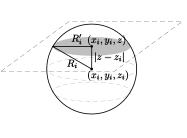
\includegraphics{fig/lnr_slice}

\includegraphics{fig/lnr_circles}
\caption{Geometry of slice in L\&R.\label{fig:slice}}
\end{figure}

The exposed arc lengths for each atom can be calculated exactly. For
each pair of atoms $i,j$, the distance between their centers projected
on the slice is $d_{ij}$ (independent of $z$). If $d_{ij} > R_i^\prime
+ R_j^\prime$, there is no overlap. If $d_{ij} < R_j^\prime -
R_i^\prime$ circle $i$ is completely inside $j$ (and the other way
around). If $d_{ij}$ lies between these two cases the angle of circle
$i$ that is buried due to circle $j$ is $$\alpha = 2\arccos
\bigl[({R_i^\prime}^2 + d_{ij}^2 - {R_{j}^\prime}^2)/(2R_i^\prime
  d_{ij})\bigr].$$ The middle point of the arc on the circle is at an
angle $\beta$ in circle $i$, and thus the arc spans the interval
$[\beta-\alpha/2,\beta+\alpha/2]$ on the circle. By adding up these
arcs and taking into account any overlap between them we get the total
buried angle $\gamma_i$ of circle $i$. The exposed arc length in this
slice is thus $L_i = R_i^\prime(2\pi-\gamma_i)$.

The contribution to the SASA from each slice is $$ S_\delta =
\sum_{i \in \text{slice}}L_i\Delta_i $$ where
$$
  \Delta_i = \frac{R_i}{R_i^\prime} \biggl[\frac{\delta}{2} 
    + \min\biggl(\frac{\delta}{2},R_i -
    \lvert z - z_i \rvert\biggr)\biggr]. 
$$ 
The factor $R_i/R_i^\prime$ comes from approximating the area of the
slice by a conical segment of the sphere, instead of a cylinder.
Finally, the total SASA is obtained by adding up the contribution from
all the slices, either for the whole protein, or atom by atom.


\subsection{S\&R}

Shrake \& Rupley's algorithm uses test points on a sphere to estimate
what parts of an atom are exposed. For each atom $i$, use a set of
test points evenly distributed (approximately) over the sphere of
radius $R_i$, and count how many of the test points are not inside any
other sphere. The number of exposed test points divided by the total
number of test points gives the exposed solid angle of that atom. The
precision of the algorithm is increased by increasing the number of
test points, and calculation time scales approximately linearly with
the number of test points.


\section{Implementation}\label{sec:imp}

This section describes the implementation of the algorithms in general
terms. In both cases the implementations are rather straightforward,
to keep them as simple and transparent as possible without sacrificing
performance. See sections \ref{sec:howto_short} and \ref{sec:using}
for instructions for how to install and use the library.

The correctness of the implementations was tested by comparing with
analytical results for the two atom case, and by performing high
precision SASA calculations using the two independent algorithms for a
large number of proteins (see section \ref{sec:dataset}) and comparing
the results. In addition, the calculated surface test
points and slice contours were inspected visually.

\subsection{L\&R}

In Sasalib, the L\&R SASA calculation begins by finding overlapping
spheres and storing the contacts in an adjacency list. For a given
slice, one needs then only check the overlap between circles that are
in the slice, and are known to potentially be in contact. The buried
arcs due to overlapping circles are calculated as described in section
\ref{sec:alg_LnR}. When all buried arcs have been counted for a given
circle they are reduced to non-overlapping intervals recursively. In
most cases only one recursion step is necessary. The lengths of
exposed arcs are then summed up for all atoms in the slice to
calculate the total contribution to the area as described in
\ref{sec:alg_LnR}.

As we will see in section \ref{sec:accuracy}, this algorithm is
significantly slower than S\&R. Profiling runs give no hints at
obvious improvements. The calculations of each slice are however
completely independent and the current implementation allows division
of labor to an arbitrary number of threads. The $O(N^2)$ calculation
of adjacency lists has not been parallelized in the current
implementation (and is a performance bottleneck in some cases). The
calculation could be both linearized and parallelized by using cell
lists, but since the adjacency lists are only calculated once for each
protein the overhead of setting up the cell lists is likely to be
prohibitive for all but the largest proteins.

\subsection{S\&R}

In S\&R the list of neighbors for each atom is only used once, hence
it is not precalculated. Generally the cost of calculating overlap
between two spheres is much larger than identifying which atoms are
neighbors, except in the limits of very few test points or very many
atoms. Calculating atom contacts on the fly also allows trivial
parallelization of the whole calculation.

Test points were generated by placing a given number of equally
charged particles on the surface of a sphere and then minimizing the
Coulomb potential using a simple Monte Carlo simulation. The obtained
sets of test-points are then stored as static arrays in a special
source file (\texttt{srp.c}), to make the program independent of any
auxiliary input files. Sets containing 20, 50, 100, 200, 500, 1000,
2000 and 5000 test points are included in the program. This set should
cover most users' need for speed and accuracy.

\subsection{Comparison of the two}\label{sec:compare}

\subsubsection{Data set}\label{sec:dataset}

For evaluating and comparing the two algorithms a list of proteins was
downloaded from the PISCES server \cite{PISCES} (on Aug 12, 2013). The
proteins have less than 20\,\% sequence identity, and the structures a
resolution of 1.6~Å or less and R-factors less than 0.25\footnote{The
  resolution of the structures is not relevant for the present
  study. It was only restricted to get a sufficiently small set of
  independent structures.}. The list specifies which chain to use in a
specific PDB-file. For the calculations here, whole PDB-files are
used, giving a larger variation in protein size, which is useful for
our purposes. The 2117 chains in the list gave a set of 2056 protein
structures used for all calculations below.

\subsubsection{Speed}\label{sec:speed}

In the limit of low precision the calculation time will be limited by
the time it takes to find which atoms are neighbors, which scales as
the square of the number of atoms. As described above this calculation
can be linearized, but with a relatively large overhead making it
worthwhile only for large proteins.

In the limit of high precision the calculation time of both algorithms
will instead scale as the number of atoms: If the number of
test-points is large in S\&R, most of the time will be spent
calculating the extent of overlap, instead of which atoms are in
contact. If there are many slices in L\&R, the calculation time will
be proportional to the number of slices, and the time of each slice
linear in the number of atoms in the slice.  The point where the
calculation time crosses over from linear to quadratic in the number
of atoms thus depends on the precision as figure~\ref{fig:time} shows.

\begin{figure}
  \begin{center}
  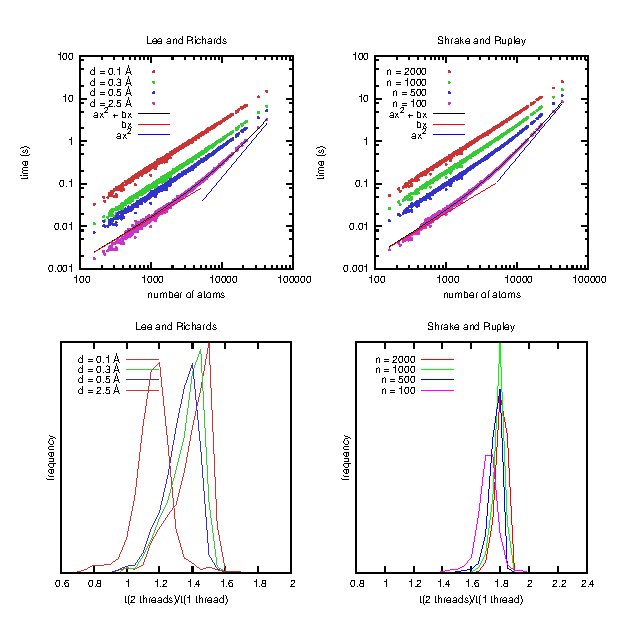
\includegraphics{fig/time}
  \caption{(Top) Calculation time as function of number of atoms for
    different levels of precision. In both cases the cross-over from
    linear to quadratic scaling as function of protein size is only
    clearly visible for the lowest precision used.  (Bottom)
    Comparison of calculation time with one and two threads, the
    histograms shows the distribution of the calculation time using
    two threads divided by the time using one thread. Thus a value of
    2 would correspond to ``perfect'' parallelization. The values
    above 2 are likely due to noise, i.e. in the very short
    simulations the timing is both inexact and might be affected by
    random factors such as background system processes.
    \label{fig:time}}
  \end{center}
\end{figure}

Where it can be done trivially, both algorithms have been
parallelized. As mentioned above, in S\&R each atom can be treated
independently, and in L\&R each slice. The efficiency of the
parallelization in a two-threaded run can be seen in figure
\ref{fig:time}. For S\&R the speed increase is close to twofold and
almost independent of the accuracy, as expected. For L\&R the
efficiency of parallelization increases with precision, i.e. the more
slices are calculated, the more there is to gain from parallelizing
the calculations. This result was also expected since the time needed
to compute which atoms are neighbors, which is done in only one thread
in the current implement, is independent of precision.

\subsubsection{Accuracy as function of speed}\label{sec:accuracy}

To measure accuracy of the two algorithms a reference SASA value,
$S_\text{ref}$ was calculated using L\&R with slice thickness
0.001~Å. The error of a given SASA-value, $S$ is then $\delta = \lvert
S - S_\text{ref} \rvert / N$, where $N$ is the number of atoms in the
protein. Figure~\ref{fig:precision} shows the results of these
calculations for the 2056 proteins described above.  It is clear from
this picture that S\&R is on average an order of magnitude more
accurate than L\&R given the same computational effort -- in the
present implementation.

\begin{figure}
  \begin{center}
  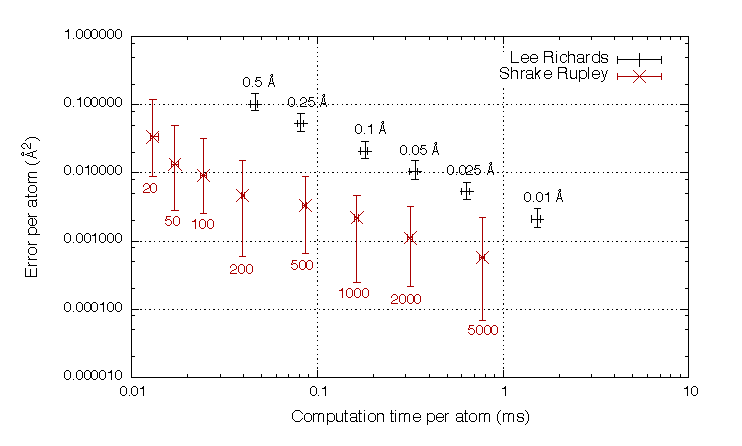
\includegraphics{fig/precision}
  \caption{The error $\delta$ in calculated SASA vs calculation time
    $t$ for the two algorithms. For the different S\&R calculations
    20, 50, 100, 200, 500, 1000, 2000 and 5000 test points were
    used. For L\&R slice thicknesses 0.01, 0.1, 0.2, 0.3, 0.5, 1.0,
    2.5 and 5.0 Å. The borders of the boxes indicate the quartiles of
    the distribution of $t$ and $\delta$ (i.e. 50~\% of the data are
    within the box), and the error bars 5th and 95th percentiles.  The
    horizontal bars are wider for S\&R because calculation time is
    less linear as function of the number of atoms than for L\&R (see
    figure~\ref{fig:time}). It is not clear why the precision varies
    more for S\&R than for L\&R.
    \label{fig:precision}}
  \end{center}
\end{figure}

\section{API} \label{sec:using}

The Sasalib API is designed to cater to the three use cases outlined
in the introduction. Therefore there are several different entry
points, giving varying degrees of control and ways of supplying atom
coordinates. Any calculation involves the following four steps.
\begin{enumerate}
  \item Initialize structure/acquire coordinates.
  \item Calculate/specify atomic radii.
  \item Calculate SASA.
  \item Output results grouping atoms/residues in different ways.
\end{enumerate}
The third step is the core functionality of the library and can be
used separately by users who wish to handle the other steps
themselves. In addition to the description below, the source for
\texttt{calc\_sasa.c} serves as an example of how to use the library,
using a large portion of the available functionality. The tests in the
directory \verb|tests| document the expected behaviour of all parts of
the API.

The header \texttt{sasalib.h} contains all functions necessary for
doing calculations with Sasalib. They wrap lower level functionality,
simplifying I/O, housekeeping, and does sanity checks on parameters,
etc. Users with specific needs can also use the functions in the
headers listed below, but these will not be documented beyond comments
in the header-files.

\begin{tabular}{r>{\raggedright\arraybackslash}p{0.7\textwidth}}
\texttt{structure.h} & Functions to deal with PDB structures,  
                       organize coordinates and other information
                       about atoms. Defines the type 
                       \verb|sasalib_structure_t|.\\
\texttt{pdb.h} & Functions for parsing inidividual lines in PDB-files \\
\texttt{coord.h} & Deals with coordinate storage and transformations. Defines
                   the type \verb|sasalib_coord_t|.\\
\texttt{classify.h} & Functions for classifying atoms according
                      to a number of different schemes.\\
\texttt{sasa.h} & Functions for actual SASA calculations, based on
                  \verb|sasalib_coord_t| objects.\\
\texttt{srp.h} & Functions to deal with test points in S\&R. \\
\end{tabular}

\subsection{Error-handling}

When an error is detected it will be reported to STDERR as an error
message prefixed with the string ``sasalib:'' and when possible a
return value indicating the severity of the error. The error-values
used are \verb|SASALIB_SUCCESS|, \verb|SASALIB_WARN| and
\verb|SASALIB_FAIL|. The first means no errors were detected; the
second that inconsistencies were detected, but calculations can
proceed, possibly with differented parameters than intended; the third
indicates more serious errors. The functions reporting calculation
results will generally return positive real values. If these detect an
error a negative value is returned, typically this involves requesting
results when the calculations have not yet been performed.  Internal
errors, i.e.\ those that are to be considered programmer errors and
not user or I/O-errors are dealt with through assert-statements. In
most cases pointers supplied as arguments to different library
functions will not be tested for validity and can thus lead to
undefined behavior\footnote{The ensuing system errors should point
  programmers using the library in the right direction.}.

\subsection{Initialization}

The Sasalib API defines one struct, \verb|sasalib_t|, that stores both
parameters and results. Coordinates stored elsewhere can be linked to
this struct to allow repeated calculations. A \verb|sasalib_t|-object
can be initalized using
\begin{verbatim}
    sasalib_t* sasalib_init()
\end{verbatim}
and the allocated resources freed using
\begin{verbatim}
    void sasalib_free(sasalib_t *s)
\end{verbatim}
The object generated by \verb|sasalib_init()| has default parameters,
and can be used directly to perform a calculation, given the correct
input. The same object can be used more than once to perform
calculations on several different proteins or different conformations
of the same protein.

\subsection{Setting parameters}

There are a number of setter- and getter-functions for specifying the
parameters of the calculations. If the specified parameter-value is
invalid the setters print an error message explaining what is wrong,
return \verb|SASALIB_WARN|, and proceed with the previously defined
value (usually the default value).

\subsubsection{Algorithms}

The following functions can be used to set and get the algorithm to be
used for a calculation. Possible values for the algorithm are
\verb|SASALIB_LEE_RICHARDS| and \verb|SASALIB_SHRAKE_RUPLEY|.  The
third function below returns the name of
the current algorithm.
\begin{verbatim}
    int sasalib_set_algorithm(sasalib_t*, sasalib_algorithm alg)
    sasalib_algorithm sasalib_get_algorithm(const sasalib_t*)
    const char* sasalib_algorithm_name(const sasalib_t*)
\end{verbatim}
The second function will always return a valid value since all
initialized \verb|sasalib_t| objects will have an assigned algorithm.

The following two functions are used to set and get the number of
points to be used in S\&R calculations. 
\begin{verbatim}
    int sasalib_set_sr_points(sasalib_t*, int n)
    int sasalib_get_sr_points(const sasalib_t*)
\end{verbatim}
And the following two set and get the slice width $\delta$ in L\&R
\begin{verbatim}
    int sasalib_set_lr_delta(sasalib_t*, double d) 
    double sasalib_get_lr_delta(const sasalib_t*)
\end{verbatim}
Finally, parameters can be copied between two \verb|sasalib_t| objects
using
\begin{verbatim}
    void sasalib_copy_param(sasalib_t *target, const sasalib_t *source)
\end{verbatim}

\subsubsection{Other parameters}
If the program is compiled in multithreaded mode the following two
functions are used to set and get the number of threads to be used in
a calculation.
\begin{verbatim}
    int sasalib_set_nthreads(sasalib_t*,int n)
    int sasalib_get_nthreads(const sasalib_t*)
\end{verbatim}
The following two set and get the name of the protein under study,
which can be useful for logging purposes.
\begin{verbatim}
    void sasalib_set_proteinname(sasalib_t*,const char*)
    const char* sasalib_get_proteinname(const sasalib_t*)
\end{verbatim}
Protein names can be no longer than \verb|SASALIB_NAME_LIMIT|
characters long. Long names are typically filenames, therefore only
the last characters of the supplied string are used if the string is
too long, assuming the omitted characters specify a path that is less
interesting than the end specifying the actual file name. The default
protein name is ``undef''.

\subsection{Calculations from PDB input}

The function 
\begin{verbatim}
    int sasalib_calc_pdb(sasalib_t *s, FILE *pdb_file)
\end{verbatim}
is used to calculate SASA for a PDB-file. The
\verb|sasalib_t|-object needs to be initialized before this
function is called. This function returns either
\verb|SASALIB_SUCCESS| or \verb|SASALIB_FAIL|. Failure can
involve both problems reading the PDB input and problems setting up
the calculations.

If the user wants to provide coordinates in some other way, but wants to
use Sasalib to calculate OONS radii, the function
\begin{verbatim}
    int sasalib_generate_radii(double **r, FILE *pdb_file)
\end{verbatim}
reads the PDB-file and calculates radii based on its contents, and
allocates memory to store them in \texttt{r}. It is up to the user to
free this memory afterwards. This function returns either
\verb|SASALIB_SUCCESS| or \verb|SASALIB_FAIL|. Failure means the
PDB input could not be read.

\subsubsection{Assumptions}

The PDB input module in Sasalib is minimalistic. Only ATOM entries are
read. If a PDB file has many MODEL entries, reading is stopped at the
first ENDMDL statement. The residue names (three-character string),
residue-numbers (four-character string), and the atom names
(four-character string) are extracted in addition to the
coordinates. This allows classification (as described below) in order
to group atoms when calculating for instance polar/apolar SASA, and
also to assign radii to the individual atoms. In the standard OONS
scheme for atomic radii, hydrogen atoms are not included, and they are
therefore excluded from SASA calculations. Users who want to include
these, and use their own set of radii will have to provide coordinates
 and radii themselves.

For simplicity, the PDB-file is assumed to be well-ordered, i.e. each
time a new residue is encountered in the file, the old one is
considered finished. This should be the case for the vast majority of
PDB files (if not all), and if not should not cause any problems,
since the residue identities are not explicitly used in the
calculation or presentation of results (only their type). 

Well-orderedness is also assumed when dealing with atoms that have
several alternate coordinates. These ATOM entries have a non-blank
value $a$ for the \emph{Alternative location indicator}. The first
non-blank encountered value of $a$ is called $a^*$, and then all
coordinates with $a = a^*$ are read. Coordinates with other values of
$a$ are ignored. When a blank value of $a$ is encountered $a^*$ is
reset.

\subsection{Atom classification and atomic radii}

Several different types of atom classification are used internally in
the library. All are based solely on the \emph{Atom name} and
\emph{Residue name} fields in a PDB file ATOM entry. These are used
for assigning atomic radii, residue type, element, OONS
type~\cite{OONS} and if an atom is polar, apolar or part of a nucleic
acid (the latter class might be divided and integrated into the former
two eventually).

Sasalib knows about the standard 20 amino acids, plus ASX, GLX,
CSE and UNK. In addition to amino acids, the nucleic acids are
identified as such, using the labels DA, DC, DG, DT, DU, DI, A, C, G,
U, I, T and N. The classification scheme was run against the entire
PDB in October 2013 and no ATOM entries not corresponding to these
classes were found. The library prints a warning when UNK entries are
found, to alert the reader that something might not be properly
defined.

For the standard 20 amino acids, and most atoms in ASX, GLX, the
regular OONS radii \cite{OONS} are used. For the unknown O or N atom in
ASX and GLX a radius of 1.5 Å is used. For nucleic acids and UNK
entries the element is deduced from the atom name and VdW radius from
www.periodictable.com is used. Atoms in UNK residues are classified as
\verb|SASALIB_CLASS_UNKNOWN|, instead of polar/apolar.

\subsection{Calculations using arrays of coordinates}

The cartesian atom coordinates are stored internally as an array of
size $3N$ and ordered as $$x_1,y_1,z_1, x_2,y_2,z_2, \ldots ,x_N,y_N,z_N\,.$$
Users that want to calculate the SASA of a set of coordinates in this form,
with corresponding atomic radii can use the function
\begin{verbatim}
    int sasalib_calc_coord(sasalib_t*, const double *coord, 
                           const double *r, size_t n)
\end{verbatim}
If the user instead wants to link coordinates to a
\verb|sasalib_t|-object to allow repeated calculations on different
conformations of the same molecule, this is done using
\begin{verbatim}
    int sasalib_link_coord(sasalib_t*, const double *coord,
                           double *r, size_t n)
\end{verbatim}

Since the library can only assign radii using PDB input the user has
to supply these as well in both the above cases. Assuming most
simulation programs can produce PDB-output, a PDB-file generated by
the caller can be used to calculate radii (using the function
\verb|sasalib_generate_radii(2)| described above) and then these
can be used as input for \verb|sasalib_link_coord(4)|. When a new
SASA values are needed these can be recalculated using
\begin{verbatim} 
    int sasalib_refresh(sasalib_t *s)
\end{verbatim}
This function returns \verb|SASALIB_FAIL| if no coordinates have
been linked using the function above.

\subsection{Results}

All the functions used to access calculated areas will return negative
values if no calculation has been performed.

The number of atoms, either supplied by the user or obtained from PDB input
is accessed by the function
\begin{verbatim}
    size_t sasalib_n_atoms(const sasalib_t*)
\end{verbatim}
The total SASA is accessed using
\begin{verbatim}
    double sasalib_area_total(const sasalib_t*)
\end{verbatim}
The integrated SASA for different classes of atoms is accessed by
\begin{verbatim}
    double sasalib_area_class(const sasalib_t*, sasalib_class c)
\end{verbatim}
where the argument \verb|c| can have the values \verb|SASALIB_POLAR|, 
\verb|SASALIB_APOLAR|, \verb|SASALIB_NUCLEICACID| or 
\verb|SASALIB_CLASS_UNKNOWN|.

To access the SASA for the different amino acid types there are two
options:
\begin{verbatim}
    int sasalib_per_residue(FILE *output, const sasalib_t *s)
    double sasalib_area_residue(const sasalib_t*, const char *res_name)
\end{verbatim}
The first prints string-value pairs of all residue types to the
specified file. All of the standard 20 residues are included, and the
other types are printed only if the SASA is non-zero.  The second
function takes the residue name as an argument and returns the SASA for
the corresponding residue. If the residue name is unknown a warning is
printed and the value recorded for the residue type ``UNK'' is
returned.

SASA of individual atoms are accessed either one by one, or
as an array of doubles:
\begin{verbatim}
    double sasalib_area_atom(const sasalib_t*, int i)
    const double* sasalib_area_atom_array(const sasalib_t*)
\end{verbatim}
and the same goes for atomic radii
\begin{verbatim}
    double sasalib_radius_atom(const sasalib_t*, int i);
    const double* sasalib_radius_atom_array(const sasalib_t *s);
\end{verbatim}
In both cases the single-valued functions return negative values if
either argument is out of bounds or there is no data available. The
functions returning pointers return NULL pointers when no data is
available.

In addition, the SASA values for individual atoms can be written as
B-factors in a PDB file:
\begin{verbatim}
    int sasalib_write_pdb(FILE *output, const sasalib_t *s);
\end{verbatim}
This function takes the PDB-file used for the calculation and replaces
the experimental B-factors with SASA-values. If coordinates are
provided by other means than PDB input the function returns
\verb|SASALIB_FAIL|. If the supplied \verb|sasalib_t|-object was first
initialized with a PDB file, and then other coordinates were supplied
through other functions, the results will however be written using the
original file if the latest coordinates have the same number of atoms
as the original file.

Finally the function
\begin{verbatim}
    int sasalib_log(FILE *log, const sasalib_t*);
\end{verbatim}
prints parameters to the file \verb|log|.

\section{Ideas for improvement and extension}

In no specific order
\begin{itemize}
\item Perl and Python bindings.
\item Other, faster or more exact algorithms.
\item Molecular surface calculations?
\item Allow HETATM-entries, if requested by user.
\item Interface to download PDB-file and calculate SASA given only PDB
  code? Is this useful?
\end{itemize}

\begin{thebibliography}{50}

\bibitem{LnR} 
  Lee B, Richards FM (1971) The interpretation of protein
  structures: estimation of static accessibility. Journal of molecular
  biology 55: 379–-400.

\bibitem{SnR} 
  Shrake A, Rupley JA (1973) Environment and exposure to
  solvent of protein atoms. Lysozyme and insulin. Journal of Molecular
  Biology 79: 351–-371.

\bibitem{OONS} 
  Ooi T, Oobatake M, Némethy G, Scheraga H (1987)
  Accessible surface areas as a measure of the thermodynamic
  parameters of hydration of peptides. Proceedings of the National
  Academy of Sciences of the United States of America 84: 3086–3090.

\bibitem{PISCES}
  Wang G, Dunbrack RL (2003) PISCES: a protein sequence culling server. 
  Bioinformatics 19:1589--1591.

\end{thebibliography}

\end{document}
